\documentclass[11pt]{article}
\usepackage[T1]{fontenc}
\usepackage[utf8]{inputenc}
% \usepackage{ebgaramond}   % house Overleaf font; commented for local tectonic build (optional)
\usepackage{microtype}
\usepackage{graphicx}
\usepackage{amsmath,amssymb}
\usepackage[margin=1in]{geometry}
\usepackage{booktabs}
\usepackage{caption}
\usepackage{xcolor}
\usepackage[numbers,sort&compress]{natbib}
\usepackage[colorlinks=true,linkcolor=teal,citecolor=teal,urlcolor=teal]{hyperref}

% AUTO-GENERATED by paper/consistency.py from reproduced, anchor-traced results.
% DO NOT EDIT BY HAND. Regenerate with: bash reproduce.sh  (or bash paper/build.sh).
% Every value traces: results/*.json -> anchors/anchors.json -> committed Gauge / CITATIONS.

\newcommand{\numDstarR}{-0.17}  % D* width-vs-repeatability Spearman r
\newcommand{\numDstarP}{0.13}  % D* Spearman two-sided p
\newcommand{\numDstarN}{76}  % same-day test-retest pairs
\newcommand{\numDstarCIlo}{-0.39}  % D* BCa bootstrap 95% CI lower
\newcommand{\numDstarCIhi}{+0.05}  % D* BCa bootstrap 95% CI upper
\newcommand{\numDR}{+0.60}  % D width-vs-repeatability Spearman r
\newcommand{\numDCIlo}{+0.42}  % D BCa bootstrap 95% CI lower
\newcommand{\numDCIhi}{+0.72}  % D BCa bootstrap 95% CI upper
\newcommand{\numCRLBgrowth}{6}  % absolute CRLB(D*) growth factor
\newcommand{\numCRLBgrowthRepro}{5.7}  % reproduced CRLB(D*) growth factor (this build)
\newcommand{\numCRLBtercileRatio}{1.12}  % high-D* CRLB(D*)/tercile-width (cohort-realized)
\newcommand{\numWidthCRLBr}{0.77}  % conformal width vs CRLB Spearman r
\newcommand{\numSunR}{0.389}  % Sun 2019 D*-Ktrans r
\newcommand{\numSunComposite}{0.533}  % Sun 2019 f*D*-Ktrans r
\newcommand{\numYangICC}{0.55}  % Yang 2019 D* reproducibility ICC
   % AUTO-GENERATED by paper/consistency.py from reproduced, anchor-traced results

\newcommand{\Dstar}{D^{*}}
\newcommand{\unit}[1]{\,\mathrm{#1}}
% Provisional marker: a claim that depends on an unpublished anchor (Fashion/Minos applied half).
\newcommand{\PROV}{\textsuperscript{\textcolor{orange}{\,P}}}
\emergencystretch=2em

% =============================================================================================
% TITLE BLOCK -- PROVISIONAL. Author list and venue await confirmation (GATE G).
% TODO-AUTHORS: confirm author list / affiliations / ORCID (default mirrors the Gauge sibling).
% TODO-VENUE:   confirm target venue (perspective). Candidates: NMR in Biomedicine (matches
%               Fashion/Lethe) or Magnetic Resonance in Medicine (matches Gauge). Class is
%               generic `article`; swap to the journal class at submission.
% =============================================================================================
\title{\textbf{The Value of a Calibrated Error Bar Is Real Where the Parameter Is
Identifiable: An End-Stage Synthesis of Trust, Value of Information, and Action in
Quantitative IVIM Imaging}}

\author{Avery Karlin\\[3pt]                                  % TODO-AUTHORS
\small Department of Applied Physics and Applied Mathematics, Columbia University, New York, NY, USA\\[1pt]
\small Department of Computer Science, University of Colorado Boulder, Boulder, CO, USA\\[1pt]
\small The Annealing Signet Institute\\[3pt]
\small ORCID: \href{https://orcid.org/0000-0003-3848-6782}{0000-0003-3848-6782}}
\date{}

\begin{document}
\maketitle

\begin{abstract}
\noindent
A deployed quantitative-MRI parameter map carries an error bar; a clinician who acts on it
faces three questions in order --- can the bar be \emph{trusted}, is a trusted bar
\emph{worth} anything to the decision, and where does acting on it \emph{break}? This
perspective synthesizes a multi-project intravoxel-incoherent-motion (IVIM) uncertainty
program into one arc, \mbox{trust $\rightarrow$ value of information $\rightarrow$ action},
and argues that the program answers the three questions as a single chain. It makes no new
measurement. The synthesis terminates in a sharp, defensible negative anchored on the
pseudo-diffusion coefficient $\Dstar$: $\Dstar$ is \emph{cross-modally orphaned}. It is
unidentifiable from its own signal --- a Cram\'er--Rao identifiability bound that grows
$\sim$\,$\numCRLBgrowth\times$ across the $\Dstar$ range and reaches the regime-bin scale in
the high-$\Dstar$ tercile (segmented IVIM, SNR\,10--100); it is un-scalable to its own
repeatability --- on real same-day test--retest data its interval width does \emph{not} track
scan--rescan scatter (Spearman $r=\numDstarR$, $p=\numDstarP$, $n=\numDstarN$; 95\% bootstrap
CI $[\numDstarCIlo,\,\numDstarCIhi]$, spanning zero), where the well-identified diffusion
coefficient $D$ does ($r=\numDR$); and it is only weakly and \emph{cohort-inconsistently}
tied to an independent perfusion readout (DCE $K^{\mathrm{trans}}$: $r=\numSunR$, $p<0.001$ in
one cohort but null in another). The end-stage caution is therefore not ``uncertainty
quantification fails'' but the sharper claim its own machinery earns: the value of a calibrated
error bar is real and quantifiable exactly where the parameter is identifiable, and $\Dstar$
marks the identifiability wall where trust, value, and action all terminate together.

\medskip
\noindent\textbf{Provisional status.} This is an end-stage synthesis assembled before its
in-program anchors have published. Claims marked \PROV{} depend on an unpublished anchor; the
load-bearing spine (the $\Dstar$ thread) rests on in-repository, reproduced anchors and survives
regardless. Submission is held until the trust and value anchors publish (Sec.~\ref{sec:hold}).
\end{abstract}

\vspace{0.4em}
\noindent\textbf{Keywords:} intravoxel incoherent motion (IVIM); uncertainty quantification;
value of information; identifiability; pseudo-diffusion; conformal prediction; decision-making.

% =============================================================================================
\section{Introduction: three questions a clinician actually asks}\label{sec:intro}
% =============================================================================================
Quantitative MRI increasingly ships not just a parameter map but an \emph{error bar} on every
voxel. The premise of uncertainty quantification (UQ) in imaging is that this error bar is
actionable --- that a clinician, or an automated triage rule, can use it to decide whether to
trust a value, escalate to another modality, or spare a patient an intervention. That premise
hides three distinct questions, and they must be answered in order:

\begin{enumerate}
\item \textbf{Trust.} Can the reported interval be believed --- does it mean what it says?
\item \textbf{Value of information.} \emph{Given} a trusted bar, is it worth anything to the
decision the clinician is actually making?
\item \textbf{Action.} When the bar is deployed and acted upon, where does it break?
\end{enumerate}

A research program is most honest when its separate results turn out to answer one question
each, and chain. This perspective makes that chain explicit for a multi-project IVIM UQ program:
a calibration ruler (the \emph{trust} anchor), a decision-theoretic pricing of a trusted bar
(the \emph{value} anchor), and two independent accounts of where deployment fails (the
\emph{action} anchors). We add no new experiment. We argue a synthesis, and we let the synthesis
fall where the evidence pushes it.

Where it pushes is onto a single parameter. IVIM models the diffusion-weighted signal as a
biexponential, $S(b)/S_0 = f\,e^{-b\Dstar} + (1-f)\,e^{-bD}$, separating tissue diffusion $D$
from a fast pseudo-diffusion compartment $\Dstar$ attributed to microvascular perfusion. $\Dstar$
is the parameter the program keeps hitting a wall on, in every one of the three questions. We use
it as the spine of the argument and call the resulting thread \emph{``$\Dstar$ cross-modally
orphaned''}: the program's whole apparatus works for $D$ (and the perfusion fraction $f$) and
collapses for $\Dstar$. Crucially, this is an \emph{identifiability} statement, not a claim that
UQ is futile. The distinction is the point of the paper.

% =============================================================================================
\section{Trust: the calibration ruler}\label{sec:trust}
% =============================================================================================
Before an error bar can have decision value it must be trustworthy: the reported interval must
have the coverage it advertises. The trust anchor (Fashion~\citep{fashion})\PROV{} builds a
model-agnostic \emph{calibration ruler} --- a check of whether a reported IVIM uncertainty is
honest --- and shows that a skew-aware posterior (an MCMC quantile interval) restores
\emph{marginal} coverage where symmetric $\pm\sigma$ intervals are miscalibrated. In its
retooled, boundary-railing-first form the ruler reports this as a scoped secondary finding under
an honest Cram\'er--Rao baseline, with the load-bearing residual being a \emph{conditional}
failure concentrated in the high-$\Dstar$ regime.

% FORWARD-CITE-fashion: Fashion is in review (NMR in Biomedicine, retooled). Code: Zenodo
% 10.5281/zenodo.20649669. No published DOI yet; cited as \citep{fashion}. Swap on acceptance.
The reading that matters for the arc: trust is achievable for $D$ and $f$, and for $\Dstar$ only
marginally --- with a residual high-$\Dstar$ hole. That hole is the seam the rest of the arc
pulls on. (This claim is \PROV: Fashion's calibration behaviour must survive review; it is a
\emph{contextual} anchor, not part of the load-bearing spine of Sec.~\ref{sec:thread}.)

% =============================================================================================
\section{Value of information: pricing a trusted bar}\label{sec:voi}
% =============================================================================================
Suppose the bar can be trusted. Is it worth anything? A calibrated interval is not automatically
decision-relevant; its value is whatever it changes about the action taken. The value anchor
(Minos~\citep{minos}) prices exactly this for a treat\,/\,spare\,/\,escalate decision, and ---
importantly for a paper built before publication --- its \emph{theory half} (the Plumbline
results) is machine-verified and publication-independent. Three results carry the section.

\paragraph{The decision--calibration gap.} The interval scale that is optimal for the
\emph{decision} departs from the scale that is optimal for \emph{coverage} whenever the posterior
is skewed and the cost is asymmetric. To leading order the gap is
$G = \tfrac{1}{6}\,|z^{*}(\lambda)|\,\gamma$, with skewness $\gamma$ and an asymmetry term
$z^{*}(\lambda)$ set by the cost ratio $\lambda$ (Plumbline Theorem~1). A symmetric problem
($\gamma=0$) or a symmetric cost ($\lambda=1$) closes the gap; IVIM is neither.

\paragraph{The value of information is second-order.} The gain from re-calibrating the bar to the
decision, rather than to coverage, is
$V = \mathrm{EU}(\tau^{*}) - \mathrm{EU}(\tau_{\mathrm{stat}}) = \tfrac12|\mathrm{EU}''(\tau^{*})|\,G^{2} = O(\gamma^{2})$
(Plumbline Proposition~3 --- the \emph{Delphi} result). The value is \emph{quadratic} in the
gap: a calibrated bar changes the decision's value only above a curvature-set ``worth-it''
floor. This is a leading-order, small-gap statement and we scope it as such --- it characterizes
the regime near the decision boundary where the quadratic approximation holds, not arbitrarily
large mis-scalings.

\paragraph{The label-free detectability floor.} A label-free validity monitor can catch
\emph{observable} distribution drift but is provably blind (AUC $=\tfrac12$) to a \emph{hidden}
channel that induces the same regret (Plumbline Theorem~2). This is the formal case that
label-free monitoring cannot, alone, certify a deployed bar; labeled spot-checks are required.

The reading for the arc: a trusted, calibrated bar has real, quantifiable decision value --- but
only where the gap is appreciable, and a label-free monitor cannot certify it by itself. The
\emph{theory} here is SOLID (independent of publication); Minos's \emph{applied} half, which
consumes the trust and action anchors, is \PROV{}. No applied number from Minos is load-bearing
for the spine below.

% =============================================================================================
\section{Action: where acting on the bar breaks}\label{sec:action}
% =============================================================================================
When the bar is deployed and acted on, two \emph{independent} walls appear --- one about the
interval's size, one about which parameter it is even possible to size.

\paragraph{Wrong size (Lethe).}\label{par:lethe}
On real same-day scan--rescan data (ACRIN-6698~\citep{acrin6698}, $n\approx76$), a conformal
interval calibrated for accuracy is far too narrow to cover real test--retest variation of $D$
(Lethe~\citep{lethe})\PROV{}. This is not a contradiction: an interval scaled for
\emph{measurement accuracy} is \emph{expected} to under-cover \emph{repeatability}, because
accuracy coverage and repeatability coverage are different targets and cannot be conflated.
Precision is not coverage. The honest-limitation verdict is sharply scoped and survives as a
caution about \emph{which} coverage a deployed interval actually provides.

\paragraph{Wrong parameter (Gauge): an identifiability wall.}\label{par:gauge}
$\Dstar$ is essentially unidentifiable per voxel (Gauge~\citep{gauge}). The argument is a
Cram\'er--Rao one and we are careful to frame it as such: the Cram\'er--Rao lower bound (CRLB) is
the smallest variance any unbiased estimator can achieve from the IVIM $b$-value curve at a given
operating point --- a statement about \emph{local identifiability}, not an impossibility proof.
Scoped to the segmented biexponential IVIM scheme and the SNR band 10--100, the CRLB on $\Dstar$
grows by a factor of $\sim$\,$\numCRLBgrowth$ across the physiological $\Dstar$ range (reproduced
in this work, Fig.~\ref{fig:crlb}; reproduced factor $\numCRLBgrowthRepro\times$), and in the
high-$\Dstar$ tercile the CRLB standard deviation reaches $\sim$\,$\numCRLBtercileRatio\times$ the
width of that tercile --- the regime is, in this acquisition, unresolvable. That conformal
interval widths track the CRLB ($r=\numWidthCRLBr$) confirms the intervals are honest about this:
they widen exactly where identifiability fails. What cannot be guaranteed label-free is coverage
\emph{conditional} on a latent axis the data do not identify --- the IVIM instance of the
impossibility of distribution-free conditional coverage~\citep{barber2021limits}, and a concrete
instantiation of the hidden, undetectable channel of Sec.~\ref{sec:voi}.

\begin{figure}[t]
\centering
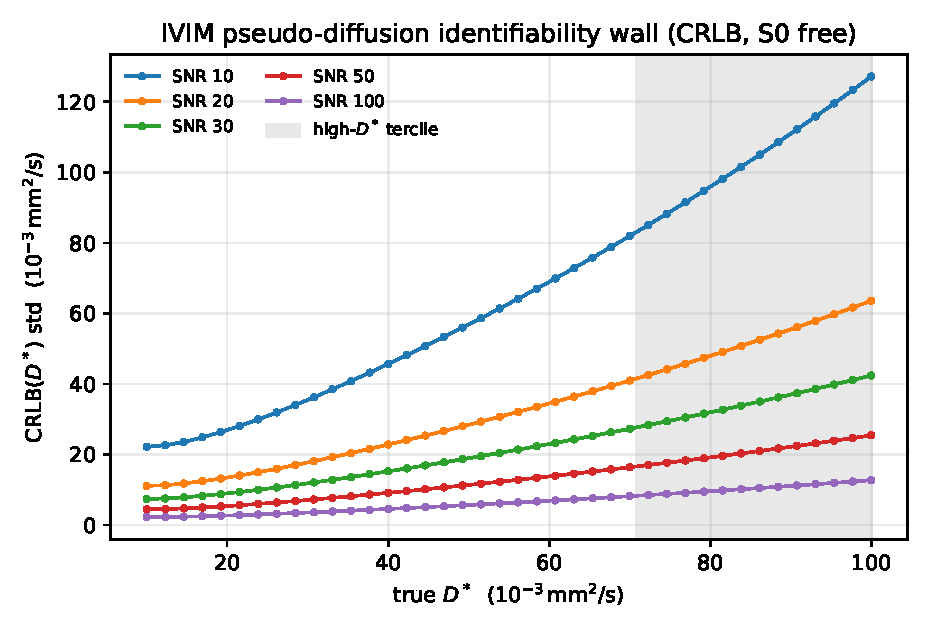
\includegraphics[width=0.74\linewidth]{../figures/crlb_wall.pdf}
\caption{The pseudo-diffusion identifiability wall, reproduced. Cram\'er--Rao lower bound on
$\Dstar$ (standard deviation, $S_0$ jointly estimated) versus true $\Dstar$ across the SNR band,
for the segmented biexponential IVIM scheme. The bound grows $\sim$\,$\numCRLBgrowth\times$ across
the $\Dstar$ range and, in the shaded high-$\Dstar$ tercile, reaches the scale of the tercile
width itself: the regime is unresolvable per voxel. This is an identifiability (CRLB) limit
scoped to this acquisition and SNR band, not an impossibility proof. Self-contained
re-derivation (\texttt{scripts/crlb\_wall.py}); cross-checked against the committed Gauge anchor.}
\label{fig:crlb}
\end{figure}

The reading for the arc: acting on the bar is safe for the parameters the program can identify
and size; it is \emph{not} safe for $\Dstar$, which sits behind an identifiability wall a
label-free monitor cannot see --- so labeled repeatability spot-checks are mandatory, not
optional.

% =============================================================================================
\section{The thread: $\Dstar$ is cross-modally orphaned}\label{sec:thread}
% =============================================================================================
$\Dstar$ is where trust, value, and action fail \emph{together}, and the failure extends beyond
IVIM, across modalities. Three independent observations form the spine. The first two are
\textbf{in-repository, reproduced anchors} (the load-bearing core); the third is corroborating
external literature.

\paragraph{(1) Unidentifiable from its own signal.} $\Dstar$ cannot be recovered per voxel from
the IVIM $b$-value curve: the CRLB grows $\sim$\,$\numCRLBgrowth\times$ in the high-$\Dstar$
regime and reaches the regime-bin scale there (Sec.~\ref{par:gauge}, Fig.~\ref{fig:crlb}). This
is reproduced from first principles in this work, not merely cited.

\paragraph{(2) Un-scalable to its own repeatability.} On the real same-day test--retest arm, the
$\Dstar$ interval width does \emph{not} track scan--rescan scatter: Spearman $r=\numDstarR$
($p=\numDstarP$, $n=\numDstarN$; 95\% BCa bootstrap CI $[\numDstarCIlo,\,\numDstarCIhi]$,
\emph{spanning zero}) --- a null. By contrast the well-identified $D$ tracks its own scatter at
$r=\numDR$ (95\% CI $[\numDCIlo,\,\numDCIhi]$, strictly positive). The $\Dstar$ null is reported
\emph{with its interval}, not as a bare point estimate, precisely because a null is only
meaningful with its uncertainty; the CI's spanning zero is the load-bearing fact. We stress the
caveat that this is a region-level, whole-tumor-ROI repeatability-tracking association on
unregistered same-day repeats --- not an in-vivo coverage, accuracy, or calibration claim. The
$\Dstar$ negative is \emph{evidence for} the identifiability thesis, not a gap in it.

\paragraph{(3) Weakly and inconsistently anchored to an independent perfusion measurement.}
If $\Dstar$ measured perfusion, it should correlate with an independent perfusion readout. The
cross-modal correlation of $\Dstar$ with DCE-MRI $K^{\mathrm{trans}}$ is, at best, weak and
cohort-dependent: $r=\numSunR$ ($p<0.001$) in one rectal-cancer cohort~\citep{sun2019} but
\emph{non-significant} in another~\citep{yang2019}, which also reports only moderate $\Dstar$
reproducibility (ICC $=\numYangICC$). We frame this honestly as \emph{weak and
cohort-inconsistent} --- significant in one cohort, null in the other --- \emph{not} uniformly
``non-significant''; both are cited. Tellingly, the composite $f\!\cdot\!\Dstar$ correlates
better ($r=\numSunComposite$), consistent with $f$ --- not $\Dstar$ --- carrying the recoverable
perfusion signal. This strand is corroborating; the load-bearing spine is (1)--(2).

\paragraph{The synthesis.} $\Dstar$ is orphaned: a trusted ruler, a priced decision, and a sized
interval all work for $D$ and $f$ and collapse for $\Dstar$ --- unidentifiable from its own
signal, un-scalable to its own repeatability, and only weakly and inconsistently tied to an
independent perfusion readout.

% =============================================================================================
\section{End-stage caution}\label{sec:caution}
% =============================================================================================
The defensible end-stage statement is not that uncertainty quantification fails. It is the
sharper claim the program's own machinery earns: \emph{the value of a calibrated error bar is
real and quantifiable exactly where the parameter is identifiable}, and $\Dstar$ marks the
identifiability wall where trust, value, and action all terminate. Operationally this is a triage
rule, and we are careful not to overclaim it at the boundary: trust the well-identified diffusion
map $D$; read high-$\Dstar$ as unresolved rather than as a measured perfusion value; price the
bar's decision value only where the decision--calibration gap is appreciable
(Sec.~\ref{sec:voi}); and, because the failing axis is one no label-free monitor can see, treat
labeled repeatability spot-checks as mandatory. None of this is a claim that $\Dstar$ ``works''
once these cautions are applied --- the spine is an honest negative, and we let it stand as one.

% =============================================================================================
\section{Provisional discipline and submission hold}\label{sec:hold}
% =============================================================================================
This synthesis was assembled \emph{before} its in-program anchors published. We treat that as a
discipline, not a disclaimer. Every claim that depends on an unpublished anchor is marked \PROV{}.
Every external number traces to a verified primary source. The load-bearing spine of
Sec.~\ref{sec:thread} --- the $\Dstar$ identifiability wall and the $\Dstar$ test--retest null
with its bootstrap CI --- rests on in-repository, reproduced anchors and is \emph{self-contained}:
the trust (Fashion) and value (Minos) projects are \emph{contextual} forward-citations, and the
core argument survives even if their final numbers shift in review. We have confirmed this
explicitly: no held or provisional number from those anchors enters the spine.

Accordingly, the manuscript is complete and reproduces green against its in-repository anchors,
but \textbf{submission is held} behind an explicit release gate until the trust and value anchors
publish (and ideally the action anchors as well). Reproduction and release are separate concerns:
\texttt{reproduce.sh} regenerates every in-repository anchor; the release gate
(\texttt{release\_gate.py}, \texttt{submit.sh}) refuses to submit while either anchor is
unpublished. The path to lift the hold, and the per-number re-check that fires when each anchor is
accepted, are documented in \texttt{SUBMISSION\_BLOCK.md} and \texttt{PROVISIONAL\_LEDGER.md}.

% =============================================================================================
\section*{Data and code availability}
% =============================================================================================
This is a synthesis; it generates no new data. The in-repository anchors are reproduced by
\texttt{bash reproduce.sh}: a self-contained re-derivation of the CRLB identifiability wall
(Fig.~\ref{fig:crlb}; \texttt{scripts/crlb\_wall.py}), the $\Dstar$ test--retest correlation
interval (\texttt{scripts/retest\_ci.py}, carrying the seeded BCa bootstrap CI and reproducing
its Fisher-$z$ twin), and the external $\Dstar$--$K^{\mathrm{trans}}$ evidence table
(\texttt{scripts/dstar\_ktrans.py}). The underlying test--retest data are the open ACRIN-6698 /
I-SPY2 breast DWI cohort (TCIA, CC-BY-4.0~\citep{acrin6698}). No private clinical data are
touched. All manuscript numbers are auto-generated into \texttt{numbers.tex} by
\texttt{paper/consistency.py} and trace to committed sources.

\paragraph{Forward-citation note.}
Fashion~\citep{fashion} and Minos~\citep{minos} are cited as in-program forward-references and are
unpublished at the time of writing; Gauge~\citep{gauge} and Lethe~\citep{lethe} are companion
manuscripts. No published DOI is asserted for an unpublished anchor; each is swapped to its
published reference at finalization per the checklist in \texttt{PROVISIONAL\_LEDGER.md}.

\bibliographystyle{unsrtnat}
\bibliography{refs}

\end{document}
